\subsection{Vòng lặp for}
\label{for}
Sử dụng vòng lặp for để lặp đi lặp loại một khối lệnh khi biết số lần lặp cụ thể. Cấu trúc vòng lặp for:\par
\texttt{for <iterator\_var> in <sequence>:}\par
	\qquad // \texttt{for block's code}\par
Trong đó:
\begin{itemize}
	\itemsep\setlength{0em}
	\item \texttt{sequence} là chuỗi hoặc collection ... cần lặp.
	\item \texttt{iterator\_var} là biến lặp, nhận giá trị của từng phần tử bên trong \texttt{sequence} ở mỗi lần lặp.
\end{itemize}
\begin{figure}[h]
	\centering
	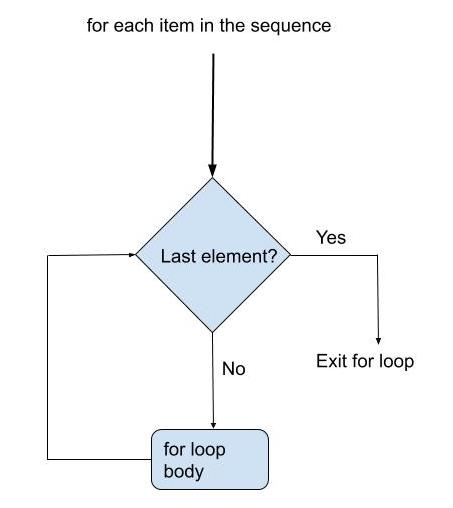
\includegraphics[width=0.5\linewidth]{img/for}
	\caption{Mô tả cách thức hoạt động của vòng lặp for}
\end{figure}
Do vòng lặp for của Python chỉ duyệt qua các phần tử có trong \texttt{sequence} nên đối với các bài toán không thao tác trên chuỗi hoặc các collections, ta phải dùng thêm hàm \texttt{range()} để trả về một danh sách các số~hạng theo thứ tự cần lặp.
\begin{table}[h]
	\centering
	\begin{tabular}{|l||l||l||l|}
		\hline
		Cấu trúc  & Giá trị & Ví dụ & Kết quả \\
		\hline
		range(n) & [0, 1, 2,... n - 1] & range(3) & [0, 1, 2] \\
		\hline
		range(x, y) & [x, x + 1, x + 2,... y - 1] & range(2, 5) & [2, 3, 4] \\
		\hline
		range(x, y, n) & [x, x + n, x + 2n,.... y'] (y' <= y - 1) & range(3, 8, 2) & [3, 5, 7] \\
		\hline
	\end{tabular}
	\caption{Mô tả kết quả hàm range()}
\end{table}
\newpage
\textbf{Ví dụ:} Chương trình nhập vào một số, tính giai thừa của số đó:\\
\rule{\linewidth}{0.2mm}\par
\begin{linenumbers}
	\texttt{n = \textcolor{red}{int}(\textcolor{blue}{input}("Type a number: "))}\par
	\texttt{factorial = 1}\par
	\texttt{\textcolor{red}{for} i \textcolor{red}{in} range(2, n + 1):}\par
	\qquad \texttt{factorial *= i}\par
	\texttt{\textcolor{blue}{print}("Factorial of \%d: \%d" \% (n, factorial))}\par
\end{linenumbers}
\rule{\linewidth}{0.2mm}\par
\noindent
\resetlinenumber
Kết quả cho ra ở Console:\\
\rule{\linewidth}{0.2mm}\par
\begin{linenumbers}
	\texttt{Type a number: 6}\par
	\texttt{Factorial of 6: 720}\par
\end{linenumbers}
\rule{\linewidth}{0.2mm}\par
\resetlinenumber
\newpage
\textbf{Ví dụ:} Chương trình nhập vào một số, tính tổng số chẵn trong đoạn [2, n]:\\
\rule{\linewidth}{0.2mm}\par
\begin{linenumbers}
	\texttt{n = \textcolor{red}{int}(\textcolor{blue}{input}("Type a number: "))}\par
	\texttt{sum = 0}\par
	\texttt{\textcolor{red}{for} i \textcolor{red}{in} range(2, n + 1, 2):}\par
	\qquad \texttt{sum += i}\par
	\texttt{\textcolor{blue}{print}("Sum of even numbers in [2, \%d]: \%d" \% (n, sum))}\par
\end{linenumbers}
\rule{\linewidth}{0.2mm}\par
\noindent
\resetlinenumber
Kết quả cho ra ở Console:\\
\rule{\linewidth}{0.2mm}\par
\begin{linenumbers}
	\texttt{Type a number: 6}\par
	\texttt{Sum of even numbers in [2, 6]: 12}\par
\end{linenumbers}
\rule{\linewidth}{0.2mm}\par
\resetlinenumber
\newpage
\textbf{Ví dụ:} Chương trình nhập vào một chuỗi, in ra từng ký tự trong chuỗi:\\
\rule{\linewidth}{0.2mm}\par
\begin{linenumbers}
	\texttt{string = \textcolor{blue}{input}("Type a sentence: ")}\par
	\texttt{\textcolor{red}{for} char \textcolor{red}{in} string:}\par
	\qquad \texttt{\textcolor{blue}{print}(char)}\par
\end{linenumbers}
\rule{\linewidth}{0.2mm}\par
\noindent
\resetlinenumber
Kết quả cho ra ở Console:\\
\rule{\linewidth}{0.2mm}\par
\begin{linenumbers}
	\texttt{Type a sentence: Python}\par
	\texttt{P}\par
	\texttt{y}\par
	\texttt{t}\par
	\texttt{t}\par
	\texttt{o}\par
	\texttt{n}\par
\end{linenumbers}
\rule{\linewidth}{0.2mm}\par
\resetlinenumber
\newpage
\textbf{Ví dụ:} Chương trình tính tổng, tích một dãy số sử dụng vòng lặp for duyệt qua các phần tử trong mảng:\\
\rule{\linewidth}{0.2mm}\par
\begin{linenumbers}
	\texttt{array = [1, 3, 5, 8, 9]}\par
	\texttt{sum = 0}\par
	\texttt{product = 1}\par
	\texttt{\textcolor{red}{for} element \textcolor{red}{in} array:}\par
	\qquad \texttt{sum += element}\par
	\qquad \texttt{product *= element}\par
	\texttt{\textcolor{blue}{print}("Sum of array: ", sum)}\par
	\texttt{\textcolor{blue}{print}("Product of array: ", product)}
\end{linenumbers}
\rule{\linewidth}{0.2mm}\par
\noindent
\resetlinenumber
Kết quả cho ra ở Console:\\
\rule{\linewidth}{0.2mm}\par
\begin{linenumbers}
	\texttt{Sum of array:  26}\par
	\texttt{Produce of array:  1080}\par
\end{linenumbers}
\rule{\linewidth}{0.2mm}\par
\resetlinenumber
\newpage
Chúng ta cũng có thể duyệt mảng bằng các sử dụng chỉ số của từng phần tử. Sử dụng hàm \texttt{len(obj)} để trả về độ dài của mảng.\par
\noindent
\textbf{Ví dụ:} Chương trình nhập vào một dãy số, tính tổng các số lẻ trong dãy:\\
\rule{\linewidth}{0.2mm}\par
\begin{linenumbers}
	\texttt{length = \textcolor{red}{int}(\textcolor{blue}{input}("Type length of array: "))}\par
	\texttt{array = []}\par
	\texttt{sum = 0}\par
	\texttt{\textcolor{red}{for} i \textcolor{red}{in} range(length):}\par
	\qquad \texttt{array.append(\textcolor{red}{int}(\textcolor{blue}{input}("Type your number \%d: " \% (i + 1))))}\par
	\texttt{\textcolor{blue}{print}("Iterating over array by index:")}\par
	\texttt{\textcolor{red}{for} i \textcolor{red}{in} range(len(array)):}\par
	\qquad \texttt{\textcolor{blue}{print}("Index \%d: \%d" \%(i, array[i]))}\par
	\qquad \texttt{\textcolor{red}{if} array[i] \% 2 == 1:}\par
	\qquad \qquad \texttt{sum += array[i]}\par
	\texttt{\textcolor{blue}{print}("Sum of odd numbers in array: ", sum)}\par
\end{linenumbers}
\rule{\linewidth}{0.2mm}\par
\noindent
\resetlinenumber
Kết quả cho ra ở Console:\\
\rule{\linewidth}{0.2mm}\par
\begin{linenumbers}
	\texttt{Type length of array: 3}\par
	\texttt{Type your number 1: 1}\par
	\texttt{Type your number 2: 4}\par
	\texttt{Type your number 3: 9}\par
	\texttt{Iterating over array by index:}\par
	\texttt{Index 0: 1}\par
	\texttt{Index 1: 4}\par
	\texttt{Index 2: 9}\par
	\texttt{Sum of odd numbers in array:  10}
\end{linenumbers}
\rule{\linewidth}{0.2mm}\par
\resetlinenumber
\newpage